\chapter{10: Operation}

\begin{abstract}
This chapter explores the nature of mathematical operations, arguing that they are not merely formal manipulations of symbols but rather expressions of embodied, normatively regulated practices. Building on the previous chapters' reconstruction of numerals as pronouns and the history of mathematical development through algorithmic elaboration, the analysis develops a framework for understanding what the author calls ``critical arithmetic''---a pre-formal system that captures the dynamic, error-inclusive nature of everyday arithmetic. Through the lens of multiplication, the chapter demonstrates how operations emerge from the interplay of three dimensions: embodied practices, inferential rules, and formal structures. The discussion begins with the embodied basis of arithmetic, using the example of a strategy called C2C (Coordinating Two Counts by Ones) documented in Cognitively Guided Instruction research. The chapter then articulates how subjective experiences are transformed into shared, rule-governed practices through a normative framework based on Robert Brandom's incompatibility semantics and the embodied cognition research of George Lakoff and Rafael Núñez. Finally, the analysis demonstrates how these practices give rise to stable, objective procedures that can be modeled as formal automata. Throughout, the chapter emphasizes that mathematical operations are grounded in human activity and social normativity rather than existing as timeless, abstract truths.
\end{abstract}

\section{The Misrecognition of Operation}

The preceding chapters reconstructed the nature of number itself, beginning with a student's profound question asked in a moment of grief and frustration: \enquote{Mr. Savich, what even is two?} That moment led away from the conventional view of numbers as abstract, pre-existing objects and toward an account of them as first-person recollective pronouns. Numerals, symbolized by the null representation $\emptyset$ (Chapter 8), emerge from the dynamic interplay of linguistic self-reference, anaphorically recollecting the enabling conditions of thought---the transcendental \enquote{I think}.

Having explored what numbers \textit{are}---reflections of dynamic, self-recollecting human being---this chapter now turns to the equally fundamental question of what it means to \textit{do} things with them. Conventional accounts treat mathematical operations as formal manipulations of abstract symbols, governed by axioms that are either arbitrary conventions or self-evident truths. In this view, addition, subtraction, multiplication, and division are processes applied to numbers, with rules to be memorized and followed.

I propose a different understanding, continuous with the emancipatory project of this book: mathematical operations are not arbitrary conventions but are themselves expressions of embodied, normatively regulated practices. The \enquote{laws} governing the use of numbers are best understood not as transcendent truths, but as algorithms or inference chains---normatively regulated doings that emerge from embodied engagement with the world and with others. This misrecognition---treating operations as mechanical procedures divorced from human meaning-making---parallels the earlier misrecognition of numbers as abstract objects divorced from the thinking subject who deploys them.

This chapter articulates inference rules for what I call \enquote{critical arithmetic}---an open-ended, pre-formal system that captures the kind of arithmetic used in everyday life---errors and all. Drawing on the empirical foundation provided by Cognitively Guided Instruction (CGI) research \parencite{Carpenter1999}, which established that children possess rich, informal mathematical knowledge long before formal instruction, the investigation reveals how mathematical operations unfold in lived experience.


\section{The First Determinate Negation: Critical Arithmetic and the Triad}

To make this misrecognition determinate, I introduce the concept of \textit{critical arithmetic}. This framework \cancel{negates} the conventional view by denying that operations exist as pre-given formal procedures. Instead, critical arithmetic reveals operations as practices that emerge through the triadic structure of validity developed throughout the inquiry.

The investigation into student-invented strategies is deeply indebted to the paradigm shift initiated by Cognitively Guided Instruction (CGI). Emerging in the 1980s from research by Carpenter, Fennema, and colleagues, CGI established that children possess rich, informal mathematical knowledge long before formal instruction \parencite{Carpenter1999}. This research provided the empirical foundation for the constructivist turn in mathematics education, asserting that students actively construct understanding by solving problems in meaningful ways, rather than passively receiving algorithms.

However, while constructivism and CGI have demonstrated significant positive effects on students' conceptual understanding, it is burdened by privileging subjective-validity claims over normative and objective validity claims. I want to use the brilliant results that emerged from the careful methods of CGI and constructivism, but reframe some of that work in a way that better integrates the triadic framework of validity developed in this book.

The primary `revision' is that strategies are not precisely `invented.' They emerge as intersubjectively constituted practices within a social context. As dyadic communicative \textit{actions} -- a speaker stakes their identity to their expressions under the assumption that someone \textit{might} be able to understand them -- they are structured by action-impeti, self-monitoring feedback loops, and existential needs for recognition. They are like orbits in intersubjective space around self-certainty, the `gravitational well'/singularity/hole in representational space. 

This revision incorporates Derridean insights into the concept of invention. At its core, invention is paradoxical: the invention must be recognized as different from what has come before, it it must also be intelligible within the existing framework of understanding.

My revision also challenges the preferred order of explanation that constructivists often employ. The tendancy is to value constructed knowledge as more valid than memorized procedural knowledge. I don't disagree with that valuation, but it isn't how I tend to learn. Instead, I tend to read/hear/observe, experience the I-feeling, as if I am genuinely recognized by what I hear, reflect, realize I have no idea what they mean, try to fit them together like a puzzle with how I understand the world, experience the I-feeling again when I take the new idea on as a commitment, and then realize the new idea is not self-certainty. 

That abstract description could stand some nuance. Take counting. A child usually learns the chant of 1, 2, 3, etc. They aren't usually counting anything, they're just repeating the chant. This is memorization, not construction. But it is a necessary step. The child must have the words in their head before they can use them to count. 

Then, through practice and social interaction, the child begins to understand that these words correspond to quantities of objects. They start to count real things, experiencing the I-feeling of successfully matching the number of objects to the last number said. This is the construction phase, where the child actively builds understanding. 

Then, eventually, they might experience the paradox of identity encoded in the claim that ten ones is one ten. This is first experienced as a falsity: ten pennies is \textit{not} one dime. There's more stuff, so they can't be the same! Then they might actually synthesize the concept of zero, realizing that, in intersubjective practices, people really do trade in ten pennies for one dime. Or they might learn to decompose a base with counting cubes. All the while, I imagine children are feeling the same sort of existential fear tracks me, like a prowling shadow, whenever I try to learn something new. Am I okay?? 


In attempting to connect the various strategies of CGI to embodied practices, bootstrapping from counting to division, the purpose is not to suggest that people actually learn so systematically. The curricula doesn't start with the breath. It started, for me, when my sister, who is two years older than I am, came home from school talking about the books she was reading. I \textit{wanted} to be as cool as she is, so I oretended to know how to read. I pretended to know how to use fractions. I pretended a lot. Eventually, I became firmly committed to communicative norms associated with mathematics. I learned to read, I learned to use fractions, and use variables. But I still don't understand why, for example, $4 \frac{m}{s^2}\times 2 s = 8 \frac{m}{s}$ -- why an accelleration multiplied by a unit of time gives a velocity. I mean, I can explain such equations using an incredibly rich vocabulary in a way that might convince a skeptic and convince anyone who doubts my understanding that I actually do understand it. But the body-feeling of accelleration accompanied by a few seconds of sitting around waiting, doesn't feel like a velocity. The reification of body-feelings as anaphoric expressions doesn't easily backfill into those same body-feelings. I don't experience speed, for example, as a body-feeling at all. Do you? You must understand that the current wisdom suggests that the solar system is orbiting the center of the Milky Way at 514,000 miles per hour. Do you \textit{feel} that? No. We feel differences---jolts in the catastrophe machine. So how would it be the case that two experiencable concepts, accelaration and waiting, multiply to give an unexperiencable concept of velocity? The best I can say is that I'm not sure. 

In any case, formalizing student-invented strategies provides some benefits. By making them explicit in a vocabulary built to describe speech-actions (formal automata), commonalities can be discerned. States and transitions may be shared across different operations in ways that the rigid adherence to the communicative norms of constructivism do not afford, precisely because of their commitment to human-centered learning. I want to be able to leverage the massive new expressive powers of computational systems to explore the space of possible strategies. This is not to say that I want to replace human-centered learning with machine-centered learning. Quite the opposite. I want to use machines to explore the space of possible strategies so that I can better understand how humans learn.

A computer, for example, can systematically explore the space of possible numbers to use in examples that might be used to invoke the crisis of strategic thinking. Right now, there are probably thousands of children working on computer-generated worksheets where the numbers being used are almost arbitrary. Yet math teachers will recognize that some numbers are more `natural' than others for teaching a concept. I liken this benefit to the problem of protein-folding. Consider how many medicines utilize proteins that were discovered by accident. Since the mid-2000s, the problem of protein-folding has been well-studied, but now machines have the capability to assist in this research, systematically exploring the space of possible proteins and their interactions. With AI, it seems possible to systematically explore the space of possible numbers to construct exemplary examples that can be used to bootstrap students' understandings into new operations. The next `phase' of math education research may include some such computationally intensive explorations.  

Consider the following example. Imagine a first-grader who can count-on, but who can't yet rearrange to make bases. Suppose they learned to count to 100 in kindergarten, and the curriculum is designed to use that prior knowledge. A computer-generated worksheet might draw from the nearly 200 million partitions of 100 to randomly select some problems. It presents the child with $15+2$. The child learns nothing, because they can count-on. Another child is randomly presented with the problem $15+7$. They are too `lazy' (in a good way) to want to do 7 inferential steps. So, instead, they draw on the material inference for object-collections that implicitly involves associativity and commutativity, to move 3 ones from 15 to 7, resulting in $12+10$, and the notion that 1 base + 1 base is 2 bases, to obtain 22. While `inventing' such a strategy takes real effort, the new structure for addition doesn't require as many monotonous inferential steps. Testing the strategy to ensure it always works requires more steps, but once the strategy has been tested, what might have taken 7 steps now only takes 3. Ideally, a teacher would serve rich problems to students, being able to tell what sorts of examples would be most likely to invoke the crisis of strategic thinking. But practically, teachers are busy. We're already letting machines do a lot of the heavy lifting in math education, but the machines are relatively stupid. They have not been trained to think about mathematics like people think about mathematics. 






These challenges motivate the need for a more structured understanding of the landscape of student-invented strategies. The formalization project undertaken here, exemplified by the Hermeneutic Calculator \parencite{savich_hermeneutic_nodate}, is not intended to restrict student invention but to rigorously analyze the strategies that emerge within intersubjective space. By treating these strategies as computational choreographies, \cancel{we} can move beyond the limitations of isolated teaching experiments and discover relationships that might otherwise remain obscured.

The triadic framework examines operations from three integrated subject positions: (1) The \textbf{subjective validity} of embodied practices, grounded in first-person lived experience; (2) The \textbf{normative validity} of inferential rules, structured through second-person commitments that exclude error; (3) The \textbf{objective validity} of formal structures, modeled as third-person automata. These three dimensions interpenetrate, forming a unity where the formal emerges from the felt, the abstract from the concrete. Operations stabilize around points of self-certainty where subjective experience, normative regulation, and objective structure achieve coherence.
\section{Systematic Analysis: The Recipe from Embodiment to Norms}

The triadic progression from subjective to objective requires a systematic recipe for moving from private, embodied feeling to shared, communicable, and rule-governed practice. This section articulates that recipe using multiplication as a running example, demonstrating how the formal emerges from the felt.

\subsection*{The Embodied Ground: Subjective Validity}

The journey of any operation begins not with a symbol, but with a doing. Children, before they are ever taught a formal multiplication algorithm, invent their own strategies grounded in embodied experience. Consider one of the most intuitive strategies: \textit{Coordinating Two Counts by Ones} (C2C). To find the total number of items in 3 groups of 4, a child counts: \enquote{one, two, three, four} for the first group, then continues \enquote{five, six, seven, eight} for the second, and \enquote{nine, ten, eleven, twelve} for the third. All the while, a second, implicit count tracks the number of groups processed.

This is a lived, felt process---a rhythmic activity grounded in the basic human capacities for grouping objects, maintaining a sequence, and tracking multiple streams of information. This represents the \textit{subjective} pole of the operation. It is a form of knowing that is inseparable from the physical act of doing, a claim to subjective validity: \enquote{this is how it feels right to me to do this.}

\subsection*{From Embodiment to Norms: The Recipe}

How do \cancel{we} move from this private feeling to a mathematical operation? The recipe unfolds in systematic steps:

\textbf{Step 1: Start with the Embodied Practice.} Begin with an intuitive strategy like C2C, grounded in subjective validity.

\textbf{Step 2: Articulate Material Inferences.} Re-describe this practice as a set of material inferential commitments using incompatibility semantics \parencite{Brandom2008}. The \enquote{goodness} of an operation is not an abstract truth but a normative status conferred upon a practice within a recognitive community. The operation $3 \times 4 = 12$ becomes a material inferential commitment:
\[
\{ \text{3 groups of 4} \} \vDash_{I} \{ 12 \}
\]

Using the definition of incompatibility entailment, this means that everything incompatible with the result `12' (e.g., asserting the result is 11 or 13) must also be incompatible with the initial premise `3 groups of 4'. By systematically excluding what is incoherent, \cancel{we} define the boundaries of coherent practice.

\textbf{Step 3: Transpose Embodied Metaphors.} Drawing on Lakoff and Núñez \parencite{Lakoff2000}, transpose their four grounding metaphors into the modal logic of Chapter 1. \textit{Arithmetic as Object Collection} grounds commutativity and associativity in the physical indifference of pooling. \textit{Arithmetic as Motion Along a Path} grounds subtraction in backward movement. These are not mere mappings but phenomenological performances---rhythms of temporal compression (reification $[T]$) and decompression (sublation $[LG]$).

\textbf{Step 4: Generate the Formal Automaton.} The result is a stable, repeatable procedure modeled as a Finite State Automaton. The automaton embodies the norms of the practice, providing a third-person, formal description. Its validity is alethic: when followed, it correctly yields results consistent with the normative framework. This is the form of the practice made explicit, a determinate structure.
\section{The Dialectical Turn: Choreography and Fractal Geometry}

Mathematical operations are, fundamentally, choreographed movements of thought. Each arithmetic strategy represents what I term \enquote{written choreography for embodied cognition} \parencite{savich_hermeneutic_nodate}. A formal automaton becomes a script for the temporal unfolding of mathematical understanding: initialize, transform, check, recurse, terminate. This framing preserves \textit{how} a student actually moves through a calculation---counting up, pausing at a boundary, decomposing a number---rather than replacing those movements with opaque symbolic shortcuts.

The dialectical turn emerges from recognizing that this choreography exhibits genuine computational self-similarity. Across twenty-five formalized student strategies in the Hermeneutic Calculator project, I consistently recover the same fractal pattern. Each strategy exhibits an \textbf{iterative core}---a minimal loop of initialize, step, and condition check---nested within a \textbf{strategic shell} that prepares, optimizes, or transforms the problem so the core runs with fewer or cognitively lighter iterations.

Consider the \textit{Sliding} strategy for subtraction. Faced with $74 - 36$, a student might recognize that both numbers can be adjusted: $(74 + 4) - (36 + 4) = 78 - 40 = 38$. This emerges from the \textit{Motion Along a Path} metaphor, where distances remain invariant under translation. The formal automaton reveals its computational structure: the strategic shell identifies a convenient adjustment value $K$ that simplifies calculation (creating a multiple of ten), then invokes the iterative core to perform the adjusted subtraction.

Strategies such as Rearranging to Make Bases, Sliding, and Distributive Reasoning wrap the iterative core with analysis that computes gaps, splits factors, or slides both numbers to maintain invariant relationships. Because the shell often invokes the core as a subroutine, the global structure becomes genuinely self-similar: strategies contain and sometimes nest earlier strategies, producing a computational fractal rather than mere metaphorical flourish.

Two fundamental movements underlie all arithmetic strategies. First, \textbf{temporal compression} (sublation/recollection) unitizes many micro-acts into larger cognitive units: ten ones become one ten, three base jumps become a single composite stride. Second, \textbf{temporal decompression} (determinate negation) strategically expands a composite to restore fine control: borrowing a ten, splitting five into two plus three, decomposing a factor for distributive reasoning. Mathematical fluency emerges as students learn to coordinate these movements, developing the capacity to know \textit{when} to expand and \textit{when} to re-compress.


\section{Second-Person Reflection: Elaboration and Formalization}

The distinction between Practical Elaboration by Training (PEdT) and Algorithmic Elaboration (AE) is crucial for understanding the structure of mathematical development. This distinction explains how mathematical understanding moves from contingent pedagogical stabilization to necessary logical elaboration.

\textbf{Practical Elaboration by Training (PEdT)} is the contingent, pedagogical process emphasized in Cognitively Guided Instruction that transforms implicit material inferences into explicit, teachable procedures. The embodied origins of mathematical concepts---the four grounding metaphors of Object Collection, Object Construction, Measuring Stick, and Motion Along a Path---require pedagogical stabilization to become reliable mathematical practices. Students must learn to count on consistently, to decompose numbers strategically, and to recognize when particular approaches are appropriate. This stabilization is fundamentally pedagogical---it depends on teaching, practice, and the social regulation of mathematical activity.

\textbf{Algorithmic Elaboration (AE)}, by contrast, represents the logical restructuring of existing abilities rather than their mere strengthening through repetition. When students reorganize their Counting On practice into the more sophisticated Rearranging to Make Bases strategy, they are not simply becoming faster counters but are discovering new inferential relationships. The elaborated strategy makes explicit what was implicit in the original practice: that numerical relationships can be preserved under certain transformations.

Strategies that stand in an LX (Elaborated-Explicating) relationship---where later practices both derive from and make explicit earlier ones---constitute what mathematics educators recognize as \enquote{conceptual understanding.} The Rearranging to Make Bases strategy explicates the associative structure latent in Object Collection. Distributive Reasoning articulates the multiplicative structure implicit in repeated addition. These relationships demonstrate how formal mathematical properties emerge from and remain grounded in embodied practice.

This second-person reflection reveals that mathematical development is not a smooth, continuous progression but involves dialectical moments where existing practices must be transcended. The failure of a strategy under certain conditions (e.g., the limitation of subtraction in $\mathbb{N}$ when facing $3 - 5$) creates the incoherence that drives elaboration toward more expressive frameworks (the integers $\mathbb{Z}$). Only after PEdT stabilizes primitive practices can AE restructure them into sophisticated strategies. The structure of mathematical development thus exhibits both contingent pedagogical moments and necessary logical transformations.

\subsection*{Formalizing Algorithmic Elaboration: Counting On to Rearranging to Make Bases}

The claim that Rearranging to Make Bases (RMB) algorithmically elaborates Counting On (CO) can be demonstrated formally through automata specifications. By examining the computational structure of each strategy, we can see precisely how the elaborated practice reorganizes and nests the primitive practice.

\subsubsection*{The Primitive Practice: Counting On}

Counting On is the foundational additive strategy. To solve $A + B$, the student starts at $A$ and counts forward $B$ times: ``$A+1, A+2, \ldots, A+B$.'' This embodies the Motion Along a Path metaphor, where numbers are locations and addition is forward movement.

Formally, Counting On can be modeled as a deterministic pushdown automaton (DPDA) with a bounded stack representing base-10 place values. The machine maintains units, tens, and hundreds on the stack, incrementing and carrying as needed.

\begin{table}[H]
\centering
\caption{\textit{Counting On Automaton ($M_{count}$).} The formal specification treats counting as iterative unit increments with automatic carry propagation (sublation) across place values. Each ``tick'' input advances the count; overflow at $U_9$ triggers temporal compression into the tens place.}
\label{tab:counting-on-automaton}
\begin{tabular}{@{}llllll@{}}
\toprule
\textbf{Current} & \textbf{Input} & \textbf{Top of} & \textbf{Next} & \textbf{Action} & \textbf{Interpretation} \\
\textbf{State} & & \textbf{Stack} & \textbf{State} & \textbf{(Stack)} & \\
\midrule
$q_{start}$ & $\varepsilon$ & $Z_0$ & $q_{idle}$ & Push($U_0, T_0, H_0$) & Initialize to 0 \\
$q_{idle}$ & tick & $U_n$ ($n<9$) & $q_{idle}$ & Pop; Push($U_{n+1}$) & Increment units \\
$q_{idle}$ & tick & $U_9$ & $q_{inc\_tens}$ & Pop & Unit overflow $\rightarrow$ carry \\
$q_{inc\_tens}$ & $\varepsilon$ & $T_m$ ($m<9$) & $q_{idle}$ & Pop; Push($T_{m+1}, U_0$) & Increment tens, reset units \\
$q_{inc\_tens}$ & $\varepsilon$ & $T_9$ & $q_{inc\_hund}$ & Pop & Tens overflow $\rightarrow$ carry \\
$q_{inc\_hund}$ & $\varepsilon$ & $H_k$ ($k<9$) & $q_{idle}$ & Pop; Push($H_{k+1}, T_0, U_0$) & Increment hundreds \\
$q_{inc\_hund}$ & $\varepsilon$ & $H_9$ & $q_{halt}$ & Pop; Push($H_0, T_0, U_0$) & Counter overflow \\
\bottomrule
\end{tabular}
\end{table}

The choreography of Counting On is simple but profound. Each ``tick'' is a bodily rhythm---a finger tap, a verbal count, a step forward. The carry operation is temporal compression: ten unit steps recollected as one ten. This primitive practice is reliable, but inefficient for larger addends.

\subsubsection*{The Elaborated Practice: Rearranging to Make Bases}

Consider my favorite example, rearranging to make bases. Remember: the formalization is not meant to intimidate---it is built to break. As my understanding of formal systems grows, the vocabularies I use to express the pragmatics of mathematical strategic thinking, the formalizations change. There is no claim to finality or completeness.

The video I analyzed is from \textcite{Carpenter1999}. The strategy descriptions and examples were adapted from Amy Hackenberg's careful reconstruction of those videos to teach pre-service teachers \textcite{HackenbergCourseNotes}. 
\begin{itemize}
\item \textbf{Teacher:} Lucy is eight fish. She buys five more fish. How many fish will Lucy have then?
\item \textbf{Sarah:}  13. 
\item \textbf{Teacher:} How'd you get 13? 
\item \textbf{Sarah:} Well, because eight plus two is ten, but then two plus three is five. And she wants to buy five more fish. So you take care of two, and you need to add three more. And so I add three more, and you get 13.
\end{itemize}

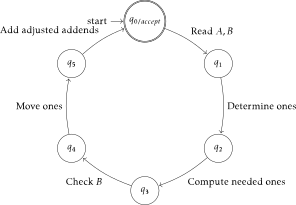
\includegraphics[width=.8\textwidth]{/Users/tio/Documents/GitHub/September_UMEDCA/images/Easy_Pictures/SAR_ADD_RMB/PDF/SAR_ADD_RMB.pdf}

\noindent \textbf{Notation Representing Sarah's Solution:}

\begin{align*}
8 + 5 &= \Box \\
8+2 &= 10\\
2+3 &= 5\\
8+5&= 10 + 3\\
8+5 &= 13
\end{align*}

\subsubsection*{Description of Strategy:}

 \textbf{Objective:} Rearranging to Make Bases (RMB) means shifting the extra ones from one addend over to the other so that one of the numbers becomes a complete multiple of the base (a whole ``group'' of that base). This rearrangement simplifies the addition process because there are established patterns for adding an exact multiple of the base. In other words, when you add a full group of base units to a number, the ones digit stays the same while only the digit representing the base (like the tens place) increases.
   


Rearranging to Make Bases transforms the counting procedure by introducing strategic planning. Instead of counting forward $B$ times, RMB recognizes that reaching the next base boundary (10, 20, 100, etc.) creates a cognitive landmark. The strategy decomposes $B$ into two parts: the gap $K$ needed to reach the next base, and the remainder $R$. Symbolically: $A + B = (A + K) + R$, where $A + K$ is a clean base.

For example, solving $28 + 7$: the gap from 28 to 30 is 2, so decompose $7 = 2 + 5$, yielding $(28+2)+5 = 30+5 = 35$. The student has reorganized the primitive counting procedure to minimize cognitive load.

\begin{table}[H]
\centering
\caption{\textit{Rearranging to Make Bases Automaton ($M_{RMB}$).} This strategy algorithmically elaborates Counting On by adding a strategic shell that computes the gap $K$ to the next base, decomposes the addend $B$, and recombines. The core counting operations are nested within this higher-level strategic structure.}
\label{tab:rmb-automaton}
\begin{tabular}{@{}lllll@{}}
\toprule
\textbf{Current} & \textbf{Condition} & \textbf{Next} & \textbf{Action} & \textbf{Interpretation} \\
\textbf{State} & & \textbf{State} & & \\
\midrule
$q_{start}$ & --- & $q_{calcK}$ & $K \leftarrow 0$; $A_{temp} \leftarrow A$ & Initialize \\
$q_{calcK}$ & $A_{temp} < $ NextBase($A$) & $q_{calcK}$ & $A_{temp} \leftarrow A_{temp} + 1$; & Count up to find \\
 & & & $K \leftarrow K + 1$ & gap $K$ \\
$q_{calcK}$ & $A_{temp} == $ NextBase($A$) & $q_{decomp}$ & $A' \leftarrow A_{temp}$ & Gap found, store \\
 & & & & new base $A'$ \\
$q_{decomp}$ & $K > 0$ & $q_{decomp}$ & $B \leftarrow B - 1$; & Decompose $B$ by \\
 & & & $K \leftarrow K - 1$ & transferring $K$ \\
$q_{decomp}$ & $K == 0$ & $q_{recomb}$ & $R \leftarrow B$ & Remainder $R$ is \\
 & & & & what's left of $B$ \\
$q_{recomb}$ & --- & $q_{accept}$ & Output $A' + R$ & Combine base + \\
 & & & & remainder \\
\bottomrule
\end{tabular}
\end{table}

\subsubsection*{The Logic of Elaboration}

Comparing these two specifications reveals the precise mechanism of algorithmic elaboration. RMB does not replace CO; it reorganizes it. The $q_{calcK}$ state uses the primitive counting operation (incrementing $A_{temp}$) to calculate the gap. The $q_{decomp}$ state uses subtraction (the inverse of counting) to split $B$. The final $q_{recomb}$ state invokes addition on the transformed problem.

The elaboration is \textit{algorithmic} because it is specifiable in principle: given mastery of counting up and counting down, the RMB procedure can be constructed through sequencing and conditional branching. It is \textit{explicating} because RMB makes explicit what was always implicit in CO---the associative structure of addition. When counting from 28 to 35, the student was implicitly crossing the base boundary at 30. RMB makes this boundary crossing explicit and strategic.

This is the structure of LX relationships throughout arithmetic. Distributive multiplication explicates the iterative structure of repeated addition. Decomposing a base (`borrowing') explicates the decomposability of place-value units. Each elaborated strategy reveals the logic that was always present in the primitive practice, transforming implicit knowing-how into explicit knowing-that.

\begin{figure}[h]
\centering
\includegraphics[width=.8\textwidth]{/Users/tio/Documents/GitHub/September_UMEDCA/images/fractal_arithmetic_iterative_core_Good.pdf}
\caption{\textit{The Fractal and Dialectical Geometry of Arithmetic.} Fractalized Arithmetic as Automata: The fractal scaling of the Iterative Core demonstrates computational self-similarity. The superimposed loops show that the Core's structure remains invariant while the scale of action changes from units to bases. The dialectical inversion (Red/Purple) visualizes how the same structure operates in opposite orientations.}
\label{fig:fractal-automata-arithmetic}
\end{figure}

The fractal architecture illustrated in Figure \ref{fig:fractal-automata-arithmetic} reveals how mathematical strategies achieve their power through self-similar structure. The iterative core---the fundamental loop of initialize, step, and check---scales across different mathematical magnitudes while maintaining its essential form. This scaling property allows strategies to work across place values, demonstrating how mathematical understanding exhibits genuine computational self-similarity. The integration of inversion (Möbius orientation flipping) with fractal nesting (core within shell) explains both the unity and diversity of arithmetic strategies: they are variations on the same underlying mathematical structure.

The formal automata do more than describe strategies; they articulate the developmental logic of mathematical understanding. They show how practices that feel natural to experienced mathematicians emerge through systematic reorganization of primitive embodied doings. They demonstrate that ``conceptual understanding'' is not a mysterious extra ingredient added to procedural skill but the capacity to articulate the inferential structure of one's own mathematical practices.


\section{Integration: The Dialectical Structure of Operations}

The concept of inversion is central to the dialectical structure of mathematical operations. The analysis reveals that operations exhibit a fundamentally dialectical relationship where opposing procedures share underlying computational structures. Subtraction strategies emerge not through the invention of entirely new procedures but through the inversion or repurposing of addition approaches.

The Missing Addend strategy reframes subtraction as forward accumulation: \enquote{What must I add to 36 to reach 74?} becomes the question structuring $74 - 36$. Counting Back mirrors Counting On, moving in the opposite direction along the number line. The Sliding strategy preserves difference across translation, maintaining invariant relationships under transformation. Borrowing reverses the carry procedure by decompressing previously sublated place-value units: where carrying compressed ten ones into one ten, borrowing expands one ten back into ten ones.

This dialectical relationship extends beyond the superficial observation that subtraction \enquote{undoes} addition. The formal automata reveal that operations often share identical computational cores while differing in their orientations or interpretations. The Möbius strip visualization captures this relationship precisely: the underlying structure (the Green core) remains invariant while the operational orientation flips between additive (Red) and subtractive (Purple) modes.

\begin{figure}[h]
\centering
\includegraphics[width=.8\textwidth]{/Users/tio/Documents/GitHub/September_UMEDCA/images/geometry_inversion.pdf}
\caption{\textit{The Geometry of Inversion: Addition and Subtraction as a Unified Structure.} The Möbius strip visualization articulates the dialectical relationship between addition and subtraction. The automata analysis demonstrates how they represent inverse orientations of the same underlying temporal structure.}
\label{fig:geometry-inversion}
\end{figure}




\section{Conclusion: Operations as Creative Possibility}

This chapter has articulated a vision of mathematical operations as embodied, normatively regulated practices that emerge from the triadic unity of subjective experience, intersubjective norms, and objective structures. Throughout this investigation, the argument has been that operations are not mere procedures applied to pre-existing objects but are expressions of human being-in-the-world.

The \textit{subjective} experience of doing (e.g., the felt rhythm of Coordinating Two Counts by Ones) provides the initial, meaningful content of an operation. It is a first-person grounding of mathematical thought, rooted in the proprioceptive and temporal structures explored in Chapter 1. The \textit{normative} framework of incompatibility semantics provides the rules of the game---a second-person structure of commitments and entitlements, defining coherence by systematically excluding error. The \textit{objective} structure of the automaton provides the formal, repeatable, and communicable form of the practice---a third-person, explicit representation of a normatively governed activity.

The critical arithmetic I propose is not a closed formal system but an open-ended, pre-formal practice that is continuously evolving through dialogue and critique. It is a practice that values the agency of learners and the creative potential of mathematical thought. It resists the scientistic impulse to reduce the rich, messy, human process of mathematical meaning-making to a single, \enquote{correct,} disembodied algorithm.

The Hermeneutic Calculator project demonstrates that student-invented strategies can be formalized without losing their connection to embodied meaning. The automata serve not as replacements for human mathematical thinking but as precise descriptions of the temporal unfolding of mathematical understanding. By treating each strategy as choreographed movement of thought, the formalization preserves rather than eliminates the human dimension of mathematical activity.

Understanding mathematical operations as embodied, normatively regulated practices reveals arithmetic not as a closed system of fixed procedures but as an open field of creative possibility. Students do not simply learn to execute predetermined algorithms but participate in the ongoing elaboration of mathematical understanding. This participation is simultaneously deeply personal---grounded in each individual's embodied experience---and thoroughly social---regulated through the shared norms of mathematical practice.

The analysis demonstrates how formal mathematical structures emerge from rather than supersede lived experience. The automata that model student strategies are not abstract computational devices but precise articulations of embodied mathematical thinking. They reveal the temporal dynamics through which mathematical understanding unfolds, showing how the formal and the felt, the abstract and the concrete, the subjective and the objective are integrated within a unified account of mathematical meaning-making.

Embracing this vision---seeing operations as a synthesis of subjective feelings, normative commitments, and objective structures---moves mathematics education toward a more emancipatory stance, fostering not just technical proficiency, but also rigorous thinking, creative exploration, and humane flourishing.


\printbibliography[heading=subbibliography]